\section{Related Work}
Over the next sections I'll present the ground work for the agent I want to achieve.
I'll start by defining what an agent is and what it needs to have/do in order to be considered social and then I'll analyse several different architectures and models that implement social agents.
Afterwards I'll present some works related to collaborative agents since it may help in the specification of my model.
I'll then conclude with a Discussion section where I'll sum up all the pros and cons of the presented works, by this point it should be clear what I'm going to use in my model and why I'm using it.


\subsection{Social Agents}
Agents represent a highly interdisciplinary field with influences and applications in several diverse areas such as economics, philosophy, logic, ecology, social science and computer science \cite{wooldridge:multiagent-systems}.
It's expectable that such a diverse field might have no universally accepted definition for agents \cite{wooldridge:intelligentagents}.

For the remainder of this section I'll, firstly, present a definition for what an Agent is and also see the notion of an intelligent agent.
I'll then continue on analysing what makes an agent social, thus defining Social Actions.
Finally, I'll move on into analysing some social agent's architectures.
By the end of this section it should be clear what requirements our agent must comply to in order to be called a social agent.

\subsubsection{Agents}
According to \cite{russell&norvig:aima}, an agent is "\textit{anything that can be viewed as perceiving its environment through sensors and acting upon that environment through actuators}".
Humans can be considered agents and so can computers.
We perceive our environment through our five senses (hearing, sight, touch, smell, and taste) and act upon it through our arms, hands, voice, etc. causing changes in the environment.
Computer programs perceive their environment through keystrokes, file contents, and network packets and act on the environment by displaying on the screen, writing files, and outputting music to the speakers, among many other sensors and actuators.

However there is a clear difference between a human being and a Unix daemon.
We do not usually think of Unix daemons as intelligent agents (although we might consider them agents).
As another example, even a light switch can be described as a very cooperative agent that invariably transmits electricity when we want it to do so; flicking the switch is the way we communicate our desire \cite{shoham:agentorientedprogramming}.
This example may sound absurd, but it is logical.

However, and following Shoham rationale in \cite{shoham:agentorientedprogramming}, considering the light bulb an agent, "\textit{does not buy us anything, since we essentially understand the mechanism sufficiently to have a simpler, mechanistic description of its behaviour}".
Therefore, it is important to understand what are intelligent agents and part from this general view of considering almost everything an agent.

In \cite{wooldridge:multiagent-systems}, Wooldridge identifies a list of capabilities that an intelligent agent is expected to possess.

\begin{description}
	\item[Reactivity] Intelligent agents must be able to respond in a timely fashion to changes in their environments.
	The environment may change while the agent is following a certain procedure, be it by the presence of other agents or by the characteristics of the environment.
	Blindly following that procedure without regard for environment changes is unwise as it may cause the agent to try to accomplish a goal that is no longer valid.
	\item[Proactiveness] Intelligent agents exhibit behaviours that will allow them to achieve their own goals. 
	\item[Social Ability] Intelligent agents are capable of interacting with other agents in order to achieve their goals.
\end{description}

As we can see, social ability is closely related with an intelligent agent's capabilities.

\subsubsection{What makes them Social?}
As we've seen, social ability is one of the main capabilities an agent must possess in order to be considered intelligent.
But what is Social Ability?
We can say that a social able agent performs Social Actions.

Consider a web browser: it exchanges messages with a web server through the Internet using a well-known protocol for communication, presenting web pages to the user on demand.
Can we consider a browser a social agent?

Even if we view both the browser and the web server as agents, this simple form of communication can hardly be considered social.
Going back to our example of Unix daemons, they are usually engaged in several exchanges of information with their peers and negotiate how to exchange this information, but that does not make them social.

As Castelfranchi puts it: "\textit{Agents are not 'agents' by virtue of the fact that they communicate;
they cannot be called 'social' because they communicate but the other way around: they communicate because they are social}" \cite{castelfranchi:socialactions}.

\begin{figure}
  \centering
    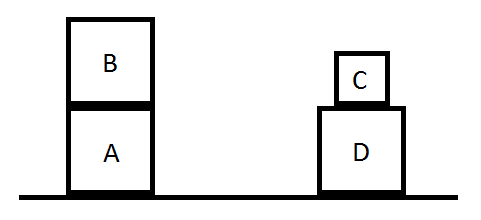
\includegraphics[width=\textwidth]{block-world-1}
  \caption{Block World initial state}
  \label{fig:block-world-1}
\end{figure}

Over the years, there as been the common misconception of considering negotiating agents as social, but as we have seen that's not always the case.
So, what makes actions social?

Imagine a block world where two agents exist, check Fig. \ref{fig:block-world-1}.
Both agents can move blocks around the world at will but cannot communicate.
The first agent, Sam, has the goal of putting both blocks A and B on the table, and the second agent, Bob, as the goal of putting block C on top of block A.
However, Bob cannot move blocks A, B, and D due to their size.
Therefore, Bob needs Sam in order to achieve its goal.

\begin{figure}
  \centering
    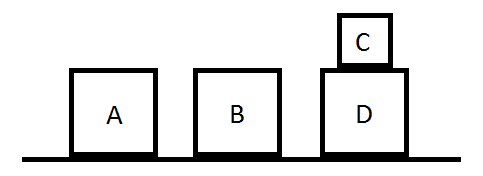
\includegraphics[width=\textwidth]{block-world-2}
  \caption{Block World after Sam's action}
  \label{fig:block-world-2}
\end{figure}

Following only its own goals, Sam will put block B on the table (check Fig. \ref{fig:block-world-2}), and Bob will then be able to put block C on top of A, completing its own goal (check Fig. \ref{fig:block-world-3}).
In this example, Sam and Bob exhibited some sort of cooperation and both achieved their own goals \footnote{This example was taken from \cite{castelfranchi:socialactions}}.

But they did so unconsciously, without knowing or having any understanding of eachother's goals, thus an action related to another agent is not necessarily social \cite{castelfranchi:individualsocialaction}.
And the opposite is also true, an action not directly related to another agent may be social in nature (consider, for example, when an agent closes a door because it doesn't want others agents looking inside the room).

\begin{figure}
  \centering
    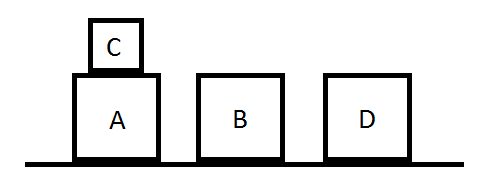
\includegraphics[width=\textwidth]{block-world-3}
  \caption{Block World final state, after Bob's action}
  \label{fig:block-world-3}
\end{figure}

To illustrate the opposite, consider two agents inside a room: the first one, John, seated at its desk and the second one, Mary, standing between John's desk and the door.
After a short conversation regarding a general topic, John, heads toward the door.
Mary, understanding John's intention of getting out of the room, promptly moves aside out of John's way, without John communicating its own intentions.

This action, of Mary stepping aside of John's way, is clearly a social one.
By interpretation of John's action, Mary demonstrated that it has an understanding of John goals and actively acts upon this knowledge.
Mary has an internal representation of John's mind, by other words, Mary is a \textit{mind-reading} agent, the basis of a social agent \cite{castelfranchi:socialactions}.

Mind-reading is the main capability an agent must posses in order to perform social actions.
And as shown in the example, this internal representation of another's agent goals and intentions, needs not be explicitly transmitted, and is, in many cases, interpreted from the agent's behaviour \cite{castelfranchi:socialactions}.

We can now understand that social agents need not only have goals and intentions of their own, but must also be able to understand and model goals and intentions of other agents.



\subsection{PsychSim}
\label{ssec:psychsim}
\begin{figure}
  \centering
    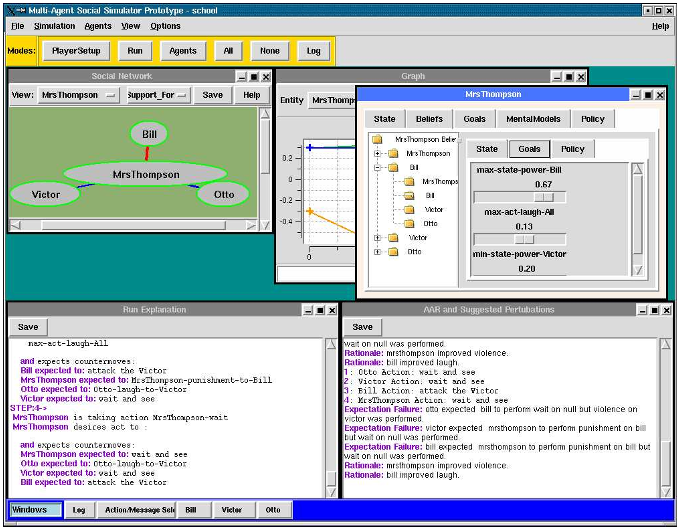
\includegraphics[width=.7\textwidth]{psychsim}
  \caption{PsychSim tool for generating new scenarios and agents.}
  \label{fig:psychsim}
\end{figure}
PsychSim \cite{marsella:psychsim} is a social simulation tool developed to explore how individuals and groups interact and how can these interactions be influenced.
The work's foundation is the fact that social interactions are based on beliefs about other's minds, a \textit{theory of mind} \cite{whiten:theoryofmind}.
Psychsim allow the users to author and explore a social scenario of his creation through the selection of generic agents models and its further specialization, see Fig. \ref{fig:psychsim}.
This tool allows users to try and understand how a specific social group might react to certain situations.

PsychSim then simulates the behaviour for each entity, individual agent or group of agents, based on their preferences, relationships, private beliefs, and mental models about each other.

In the given example, the authors explore a bullying scenario in a school and try to answer several questions:
"\textit{How might a bully respond to admonishments, appeals to kindness or punishment? 
How might other groups react in turn? 
What are the predictions or unintended side effects?}".
The simulation tool then provides explanations of the results based on each entity's preferences and beliefs, allowing the user to answer the previous questions.

PsychSim's agents are empowered with fully specified models of each other \cite{pynadath:modellingtheoryofmind}, a unique aspect of its design. Every agents maintains independent beliefs about the world, has its own goals, and it owns policies to achieve those goals. The model is composed by the state, actions, goals, beliefs, policies, messages, and mental models.

\begin{description}
\item \textbf{State} Each agent model includes a state with facts about the world, some of which may be hidden from the agent.
\item \textbf{Actions} Agents have a set of actions they can perform. Each action consists in an action type, a performer, and possibly an object of the action.
\item \textbf{Goals} These represent an agent's incentives for behaviours. In PsychSim, goals are reward functions that map the current state to a real value.
\item \textbf{Beliefs} The simulations agent have only a \textit{subjective} view of the world, where they form beliefs about what \textit{they} think is the state of the world. An agent's beliefs consists in models of all agents (including himself), representing their state, beliefs, goals, and policy of behaviour.
\item \textbf{Policies} Each agent's policy is a function that represents the process by which it selects an action or message based on its beliefs and goals.
\item \textbf{Messages} Messages are attempts by one agent to influence the beliefs of recipients and have five components: a source, recipients, a message subject, content, and overhearers.
\item \textbf{Mental Models} An agent's beliefs about another agent are realized as a fully specified agent model of the other agent, including goals, beliefs, and policies. Mental Models are predefined models which represent agents goals, beliefs, and policies.
\end{description}

As a social agent architecture, PsychSim presents a well-defined model capable of fully simulating social behaviour.
It is based on sound theories from psychology (theory of mind) and has into account other agents in its cognitive process, a requirement for social agents as we saw in \ref{ssec:social-agents}.

However, PsychSim lacks planning capabilities.
Based only of policies to guide it's immediate behaviour, each agent will follow the scenario devised by the user disregarding any future states.
\subsection{Comme il Faut}
\ac{CiF} is an \ac{AI} system that enables authors to create interactive stories by specifying, not the complete narrative and all its ramifications but, high-level rules governing expected character behaviour given social situations \cite{mccoy:cif-social-story-worlds}.
In \ac{CiF}, characters use many attributes of the current social state, including the story of prior interactions, to decide how to engage in social exchanges with other characters.
This architecture provides a rich social environment for characters to interact allowing the creation of dynamic and interactive stories.

\ac{CiF} does not store world information in a series of events, like many \ac{AI} techniques do (e.g. Behaviour Trees and Hierarchical Task Networks).
Social exchanges are the primary structure of representing knowledge in \ac{CiF} \cite{mccoy:cif-authoring}.
They consist in social interactions between characters that modify the social state of the participants.
By using social exchanges and additional encoded social context, \ac{CiF} lowers the authoring burden needed to create the social aspects of an interactive story by allowing the author to specify the rules and general patterns of how social interaction should take place.

Characters' behaviour is chosen based on rules in a large rule database that depict normal social behaviour in a particular story world.
These rules in conjunction with the logic of a social world, a set of characters, and a series of scenario goals allows \ac{CiF} to determine the desired action for each character.

\ac{CiF} provides a sound model for empowering characters with social ability, but it's main goal is storytelling.
As an architecture for an agent, it lacks planning capabilities that we need for our agent.
Despite its successful implementation in the game Prom Week \cite{mccoy:prom-week} \footnote{Mismanor, a still in development role-playing game that uses an altered version of \ac{CiF}, is another example.}, the authors still need to specify every rule for every possible social interaction between characters. Prom Week contains over forty nine hundred unique influence rules, around sixty social exchanges with over twenty rules that contribute to the characters desire and responses, a cast of eighteen characters, and a combined total of over forty thousand predicates.
\subsection{Fatima}
\subsection{Versu}
Versu is a text-based interactive drama available in the App Store for the iPad\footnote{You can visit the game webpage at https://versu.com.}, see Fig. \ref{fig:versu}  \cite{evans:versu}.
One of the game's appeal is its high re-playability due to the use of autonomous agents (the user can play the same episode several times with different results).

\begin{figure}
  \centering
    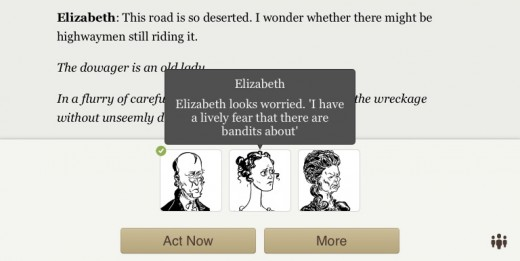
\includegraphics[width=.7\textwidth]{versu}
  \caption{An example of Versu's game play.}
  \label{fig:versu}
\end{figure}

The game is based upon two objects: agents and social practices.
Social practices describe a recurring social situation that may exist only for a short time (e.g. a conversation, a game, a meal) or can last much longer (e.g. a family, the moral community).
These practices coordinate agents via the \textit{roles} they are playing and their main function is to describe the actions the agents can do in each situation.

Social practices provide the agent with a set of suggested actions, but it is up to the agent himself to decide which action to perform, using utility-based reactive action selection (the utility is calculated in accordance with the agents beliefs, desires, personality quirks, and backstory).

Versu's world allows multiple practices to exist concurrently. For example, in a dinner party, there will be multiple practices operating at once:
\begin{itemize}
\item eating and drinking.
\item the conversation about politics
\item the rising flirtation between Frank and Lucy
\item responding to the fact that Mr. Quinn has spilled the soup.
\end{itemize}

Performing an action can result in any sentence being added to the world database.
The results of adding new sentences can be that relationships are updated, new beliefs or desires are formed, old practices are deleted or new practices are spawned.

Agents and social practices are scripts authored in a high-level \ac{DSL} designed specifically for this simulation: Praxis\footnote{Praxis is based on Exclusion Logic \cite{evans:exclusion-logic}, a new deontic logic.}.

Versu's success is proof that the architecture can produce social agents with high adaptability.
But, as some of the already explored works, Versu's agents lack planning capabilities.
It's logic powered approach is a differentiating aspect from the previous models, however it does imposes some limitations.
One example is how the agents beliefs are expressed.
The system cannot represent universal and existential quantifiers (e.g. "everyone has become insane" and "the murderer is one of the guests", respectively) or beliefs about others' beliefs (e.g. "Mr Quinn believes that Lucy believes that Mrs Quinn is the murderer").

\subsection{dorgoly-social-agents}

\subsection{Colaborative Agents}
Given the nature of the environment I'm working with (a multi-agent environment), it may be of special interest to understand and explore works based on collaborative agents.
Although the agent may not always collaborate, collaboration will be a major point of the agents' activities since most of the interactions with other players will occur during collaboration.



\subsection{Discussion}
Throughout the previous sections we've looked at social agents and some works that use and implement social agents.
We've also taken a look at collaborative agents with the purpose of defining a model to implement a social agent.

There are several aspects that an agent must possess in order to be considered social, as discussed in \ref{ssec:social-agents}.
Keeping in mind that the agent's actions must be social by design, the key capability of a social agent is mind-reading.

All of the explored architectures have mind-reading capabilities provided by the use of \ac{TOM} models.
\ac{TOM} models allow the agent to include other agents perceived intentions and desires in its deliberative process (either in choosing a single action or in a planning processes).
So what differentiates them?

One of the main points argued was the planning capabilities of the architectures/models.
As we've seen, PsychSim, \ac{CiF}, and Versu lack this ability while \ac{FAtiMA} and Dorgoly's architecture don't, making them better suited for the agent.

Although it was not a requirement, both \ac{FAtiMA} and Dorgoly's architecture made use of appraisal theories to model emotions.
This is not at all bad for the agent's purpose, as it can help the players to better relate with it.

Finally, Dorgoly's architecture distinguishes itself from \ac{FAtiMA} by its use of roles to model social context, although \ac{FAtiMA} could also achieve social behaviour through the use of another module, Dorgoly's architecture already includes all that logic in its core processes, making it, in my opinion a stronger model for this problem.
